\subsubsection{Setup}

The first thing we did was decide how to structure our code. We took a lot of inspiration from \href{https://github.com/IvanGeffner/BTC24}{XSquare's 2024 code}. We created an abstract \verb|Robot| class, and created a subclass for each robot type (\verb|Soldier|, \verb|Splasher|, \verb|Mopper|, \verb|Tower|). This heavily simplified our \verb|RobotPlayer| class, and helped us split functionality between differing robot types\footnote{In hindsight, it may have been even smarter to have another level to the hierarchy where we had Unit as the base class, Robot and Tower as subclasses, and other types inherit from these. Towers don't need to do pathfinding, and they can't really learn much about the map, so this was bad organization and wasted bytecode}. Along with these classes, we also had utility classes, like \verb|MapData|, \verb|Explore|, \verb|Bugpath|, and others.

\medskip

Our first priority was getting a bot that could effectively explore and capture towers. Building towers would allow our team to increase their resource income and create more robots. We had each tower spawn a soldier and a mopper who would search for a ruin. We copied the capture logic from examplefuncsplayer. The soldier was to paint the pattern around the tower, and the mopper was to clear any enemy paint in the way.

\subsubsection{Resources \& Towers}

We made two observations very early on about resources:
\begin{enumerate}
  \item It is not worth upgrading towers.
  \item It Money towers are always better than Paint towers.
\end{enumerate}
The first one is relatively obvious looking at the costs of new towers vs upgrades. For Money towers, the following table shows the cost associated with each level of the tower:
\begin{center}
  \begin{tabular}{c | c | c}
    Level & Upgrade Cost (Chips) & Mining Rate (Chips / Turn) \\
    \hline 
    1 & 1000 & 20   \\
    2 & 2500 & 30   \\
    3 & 5000 & 40   \\
  \end{tabular}
\end{center}
From this table, we can graph the cost and mining rates:
\begin{center}
  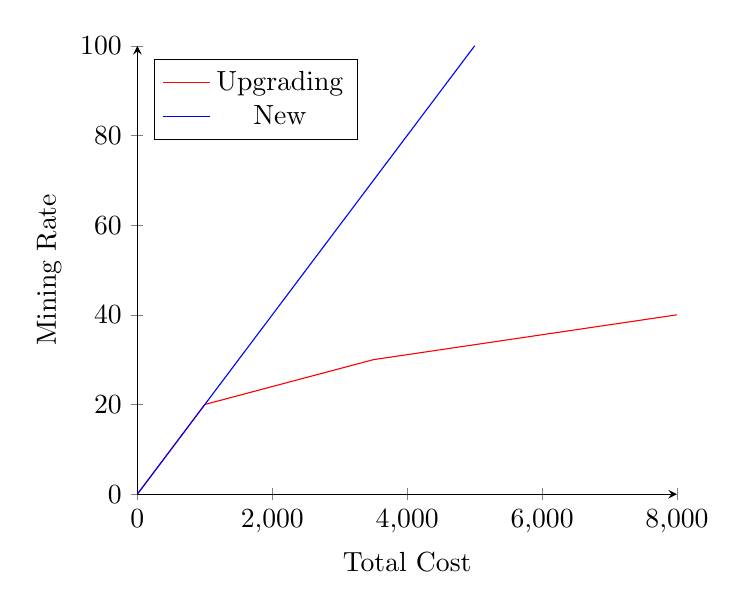
\begin{tikzpicture}
    \begin{axis}[
      axis lines = left,
      xlabel = Total Cost,
      ylabel = Mining Rate,
      legend pos = north west
    ]
    \addplot [
      color = red
    ]
    coordinates {
      (0,0)(1000,20)(3500,30)(8000,40)
    };
    \addlegendentry{Upgrading}

    \addplot [
      color = blue,
      domain = 0:5000
    ]
    { x / 50 };
    \addlegendentry{New}
      
    \end{axis}
  \end{tikzpicture}
\end{center}
As is clearly shown here, when you have the choice between spending on a new tower, or upgrading an existing one, there is no reason to upgrade. The same can be said for Paint towers, but the next observation makes that redundant.

\medskip

Even though paint is arguably the more important resource, Paint towers are useless\footnote{This is true until you factor in SRPs, but we are getting there} because money towers actually produce paint more effectively than paint towers. Each tower spawns with 500 paint. Since money towers produce 20 chips per turn and they cost 1,000 chips, they pay for themselves in 50 turns. So, if a Money tower calls \verb|rc.disintegrate()|, we can trade 1,000 chips for 500 paint. If we do this every 50 turns, money towers have an effective paint mining rate of 10 paint per turn, which is double what paint towers are capable of.

\medskip

Here is the corresponding graph to the above for paint production vs chip cost:
\begin{center}
  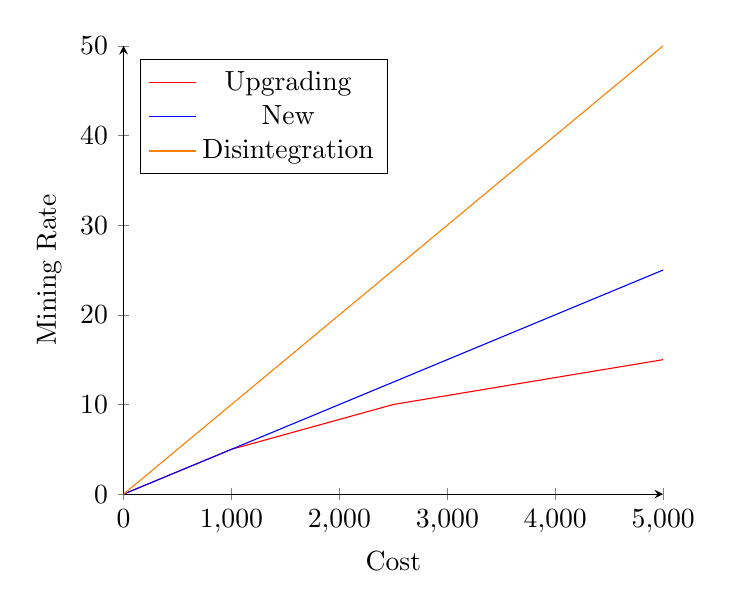
\begin{tikzpicture}
    \begin{axis}[
      axis lines = left,
      xlabel = Cost,
      ylabel = Mining Rate,
      legend pos = north west
    ]
    \addplot [
      color = red
    ]
    coordinates {
      (0,0)(1000,5)(2500,10)(5000,15)
    };
    \addlegendentry{Upgrading}

    \addplot [
      color = blue,
      domain = 0:5000
    ]
    { x / 200 };
    \addlegendentry{New}
    
    \addplot [
      color = orange,
      domain = 0:5000
    ]
    { x / 100 };
    \addlegendentry{Disintegration}
    \end{axis}
  \end{tikzpicture}
\end{center}
There are a few other big bonuses of this strategy:
\begin{enumerate}
  \item We now have the choice of converting chips to paint. With paint towers, if we have more paint than we need or can use, we are stuck with it.
  \item We no longer have to coordinate what tower types we are building, since we are always building money towers (we ignore defense towers for now).
  \item Since chips are global and paint is local, we can use money towers that are far away from the active parts of the map to subsidize paint production where it is needed most.
\end{enumerate}
With this, it made a very useful optimization trivial. Marking a tower pattern costs 25 paint, which is significant considering the soldier's paint capacity is 200, and it already takes a minimum of 120 paint to capture a ruin. Since we knew we were only building money towers, we could avoid marking the pattern and save paint.

\medskip

As a side note, we thought this strategy was pretty well known, however this ended up winning Gone Whalin' the ``Most Innovative Breakthrough Prize'', and most teams noticed it when they started doing it right before US Qualifiers. Overall they simply had a much better bot than us, holding a pretty stable rating around 1900.

\subsubsection{Special Resource Patterns}

Once SRPs are introduced, the math on paint production changes. Each active SRP boosts paint production by 3 units per tower per turn. The following table shows how the number of SRPs affects the per turn production rates of different towers:
\begin{center}
  \begin{tabular}{c | c | c | c}
    SRPs & Money Tower Chips & Money Tower Paint & Paint Tower Paint \\
    \hline
    0 & 20 & 10 & 5 \\
    1 & 23 & 11.5 & 8 \\
    2 & 26 & 13 & 11 \\
    3 & 29 & 14.5 & 14 \\
    4 & 32 & 16 & 17 \\
    5 & 35 & 17.5 & 20
  \end{tabular}
\end{center}
As you can see, once there are 4 or more SRPs, paint towers are better suited for their intended purpose. We decided not to worry about this and stick with our money tower only strategy, to keep things simple. Plus, we (regrettably) did not prioritize SRPs for Sprint 1, our soldiers simply checked if the current location could have an SRP and if so, they marked one.

\subsubsection{Pathfinding \& Map Representation}

Units stored their knowledge of the map in memory, however we ended up rewriting this system, so this will be described further later. Units traversed the map using a BugNav algorithm. We used the BugNav algorithm from \href{https://github.com/IvanGeffner/BTC24/blob/master/BugPath.java}{XSquare's 2024 code}, and it worked with minor tweaking. If you have questions about how to implement this, there was a lecture on it this year \href{https://www.youtube.com/live/Mqk50BQH3oQ?si=6qL5WAXmSOS2K3OR}{here}.

\medskip

Optimal pathfinding wasn't a high priority this year since ruins/towers guaranteed a lot of open space, and the specs guaranteed walls to take up less than 20\% of the map. In theory, Teh Devs could've made maps with few ruins and many walls, but that never happened. Even though something like unrolled BFS would've been optimal, BugNav worked well enough in practice, and because source code for it already existed, we saved a lot of time not worrying about pathfinding.

\subsubsection{Sprint 1 Performance}

The bracket for Sprint 1 can be found \href{https://challonge.com/bc25javasprint1}{here}.

\medskip

We entered the tournament as the 55 seed out of 160 teams, with a rating of 1533, our first match was a 4-1 win against the 74 seed, ``be right back'' with a rating of 1483. Their strategy was to do an early rush with soldiers to try and take out our towers, then produce a single splasher to cover some paint. This worked against us on the first game, as our starting soldiers got stuck trying to capture an SRP with enemy paint, and our moppers didn't help them.

\medskip

The left image below shows the result of our loss, and the right image shows one of our wins. On this particular map, the opponent's rush got trapped against a wall, allowing us to expand freely.
\begin{center}
  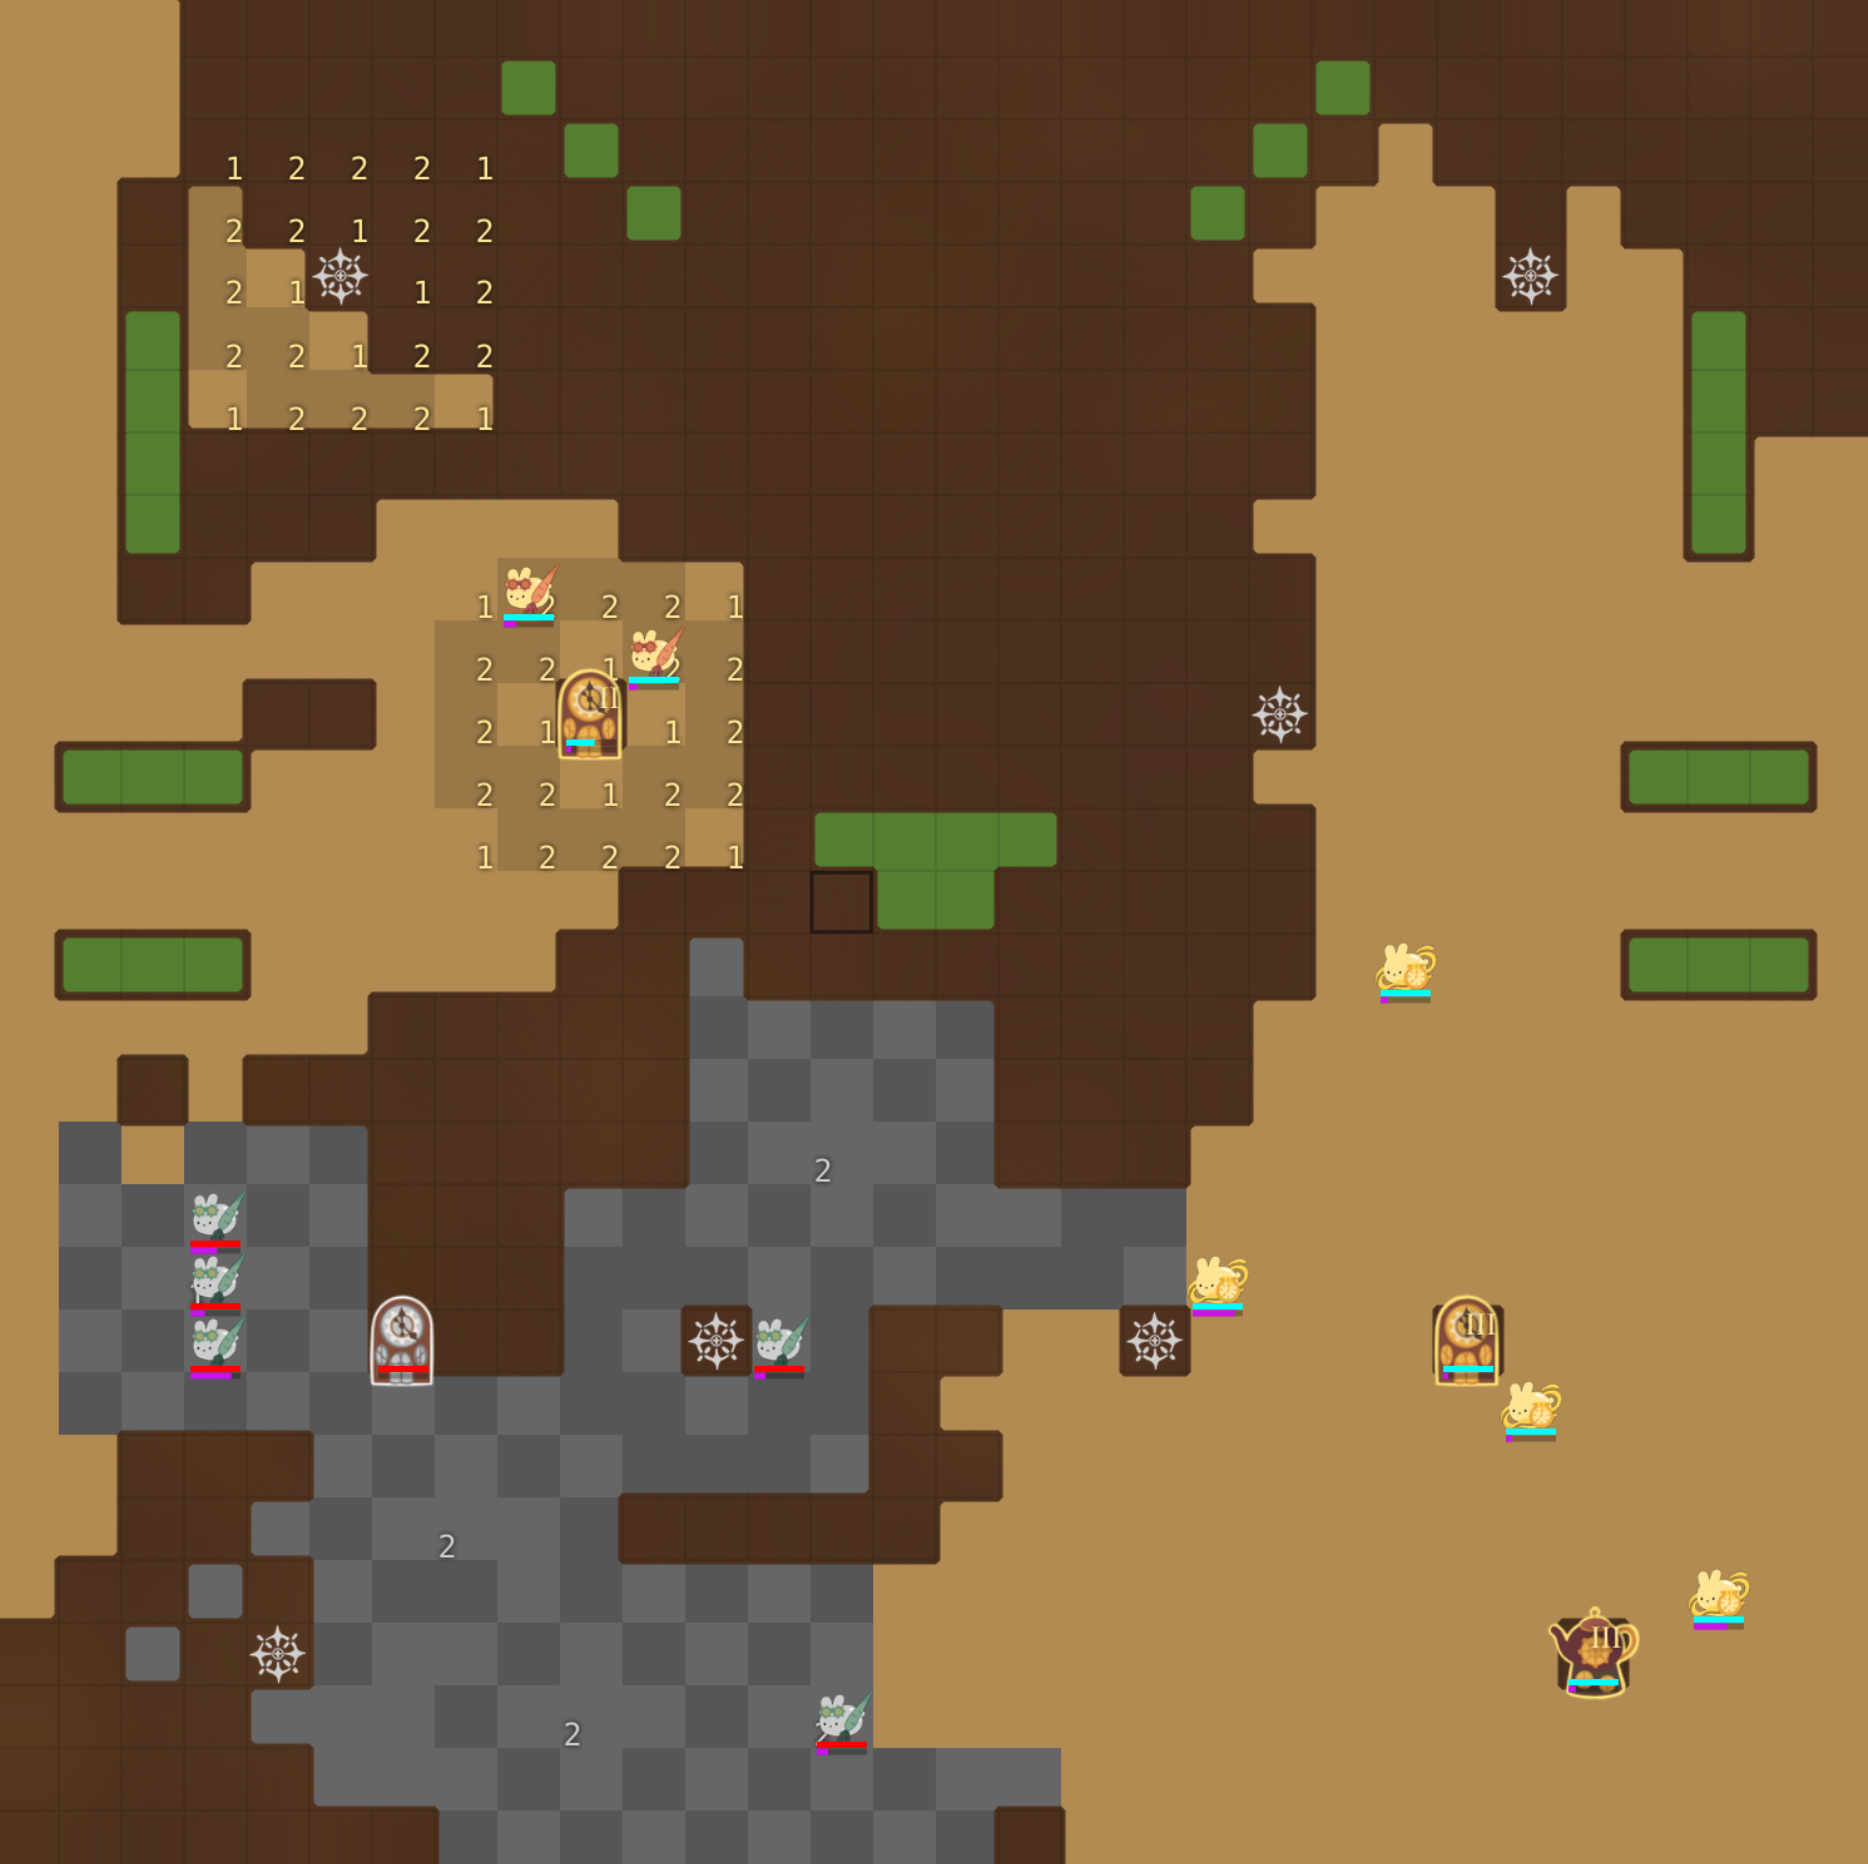
\includegraphics[scale=0.1]{images/sprint1_loss.png}
  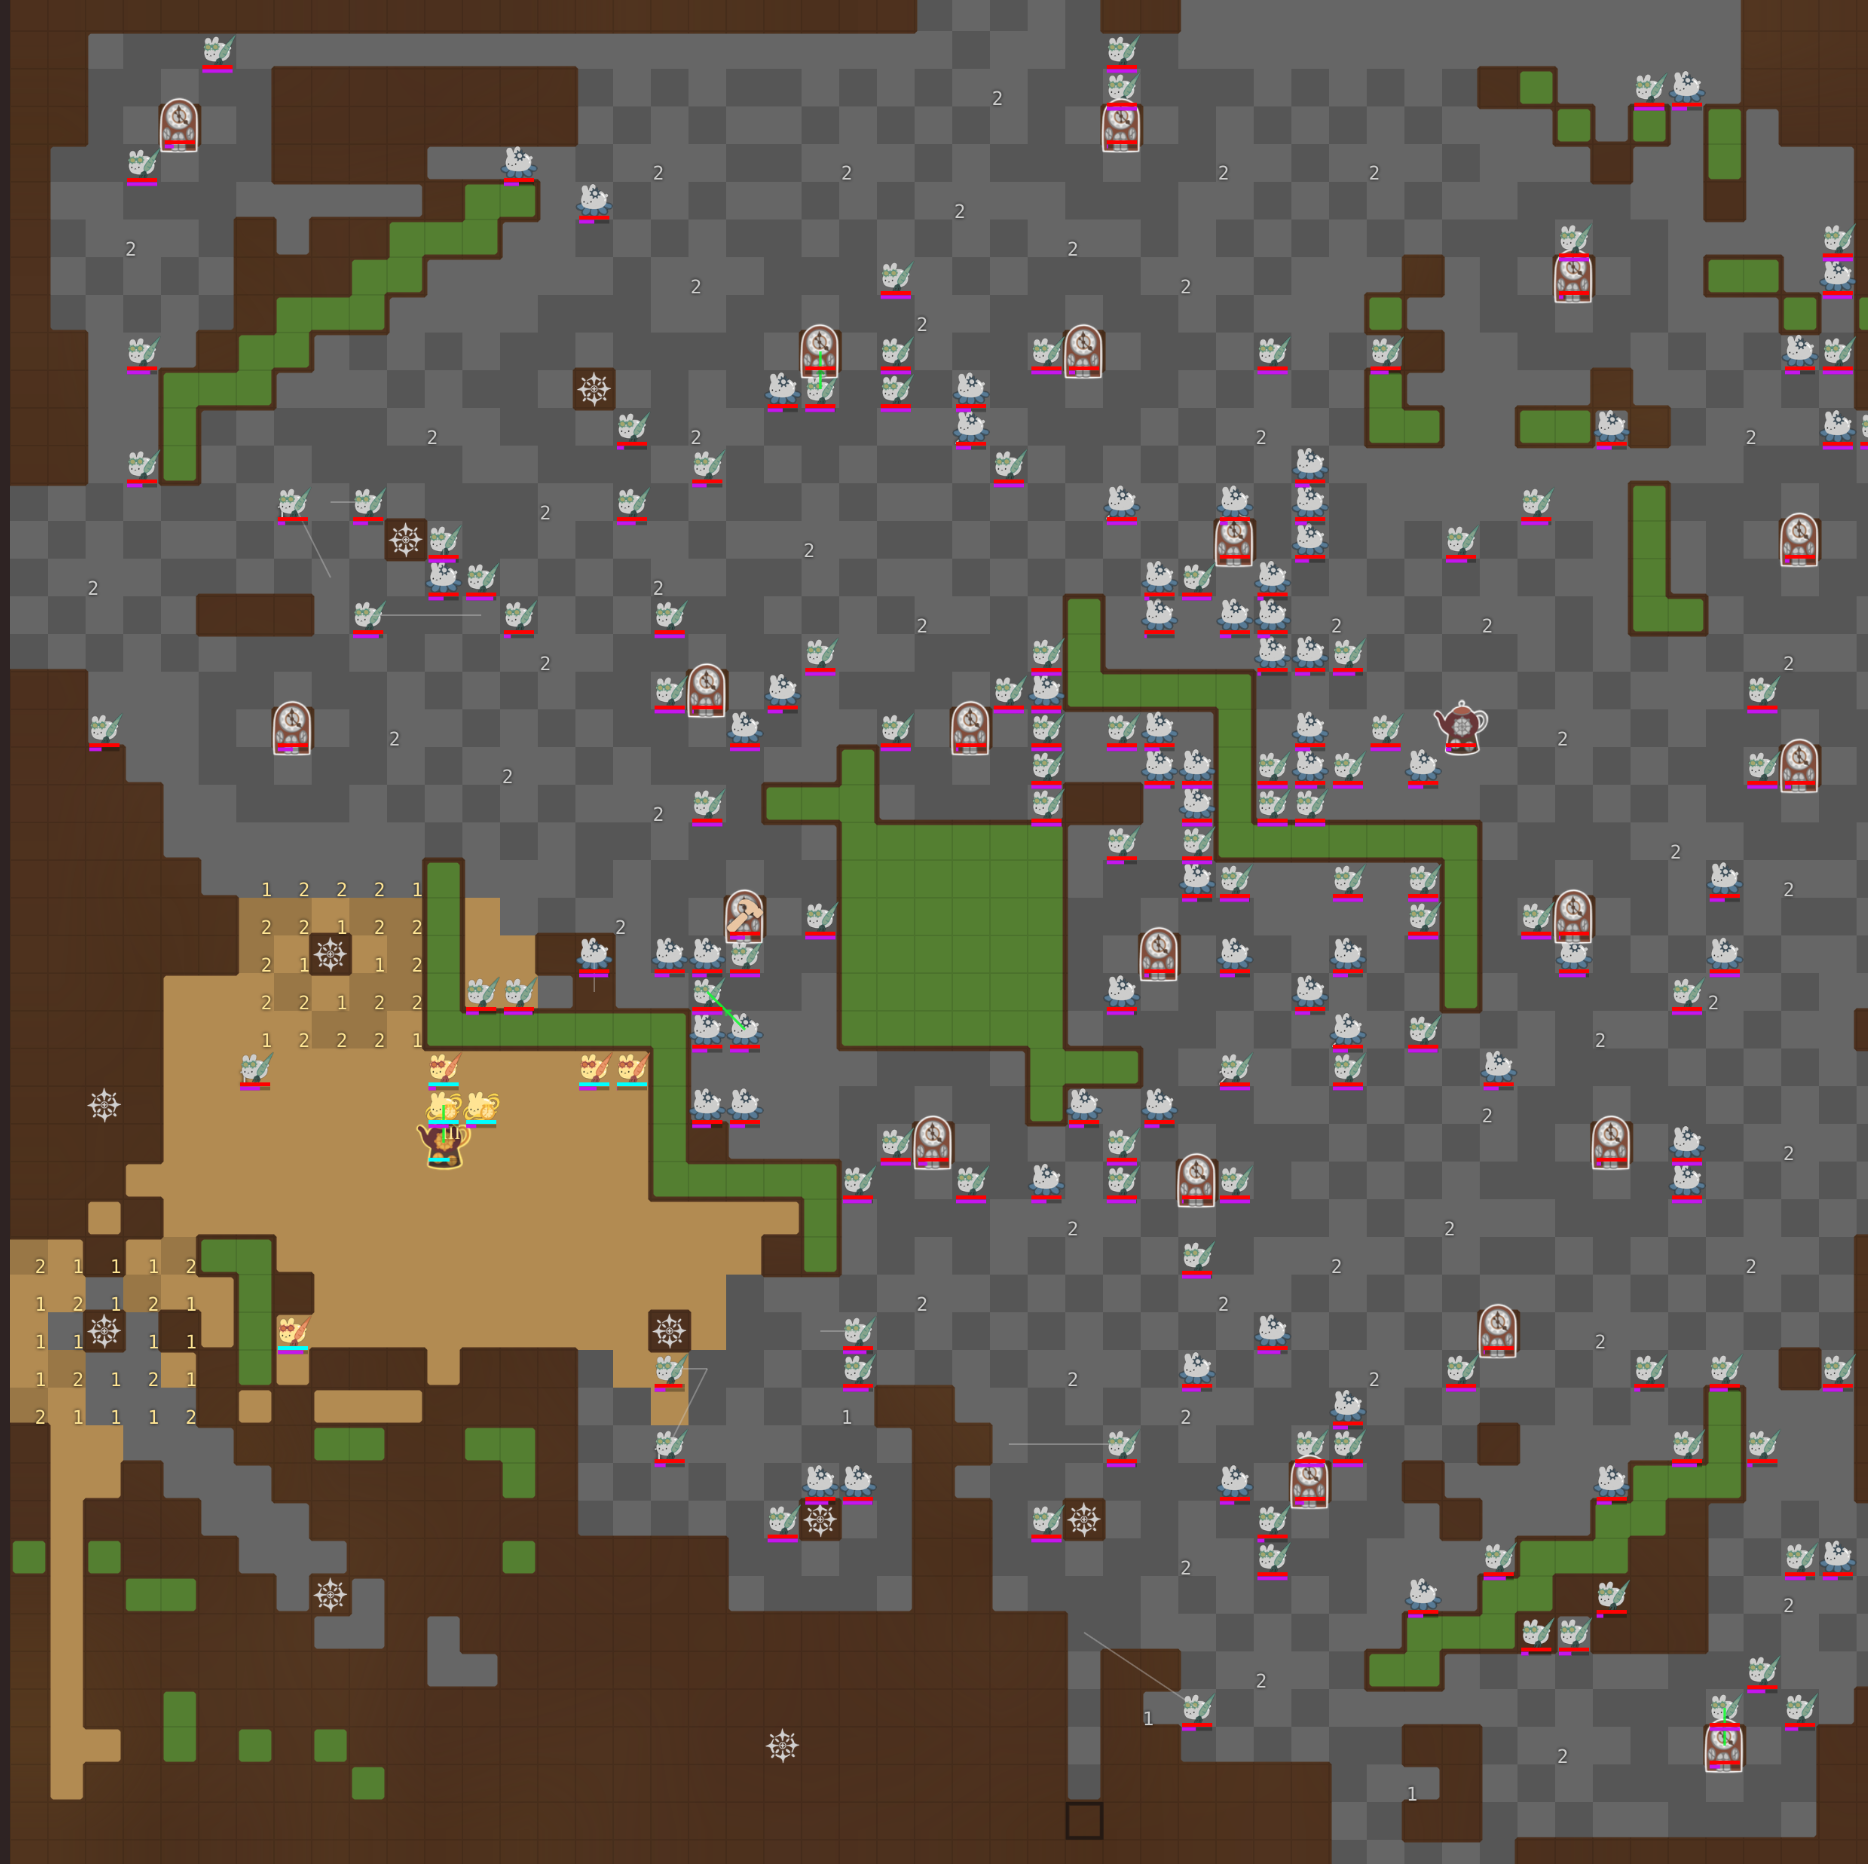
\includegraphics[scale=0.1]{images/sprint1_win.png}
\end{center}
Our next matchup did not go as well for us. We faced against the 10 seed ``immutable'', who was had a rating of 1737 at the time, and got swept 5-0. We kept up in the early game, our initial soldiers seemed to perform about equally in finding ruins, but after some starting territory was established, they always pulled away with a commanding lead. There were three main reasons for this:
\begin{enumerate}
  \item They prioritized SRPs heavily. In Sprint 1, this was definitely the meta, since the pattern allowed for an absurd amount of overlap, and there was no cost to making them. This gave them a much stronger economy than ours.
  \item They used their economy better, settling around 50\% soldiers, and 25\% each of moppers and splashers. We usually ended up with about even soldiers and moppers with no splashers, since we did not have time to create splasher logic by this point. Their balance allowed for much better expansion.
  \item They explored the map better. Our soldiers would often get stuck on ruins they couldn't complete without help, and our moppers were terrible at finding soldiers to help. This meant we got stuck anytime we saw enemy paint.
\end{enumerate}
We are sure there are many other things they did better than us, but these were the three big differences that made the others negligible.